\documentclass[14pt]{beamer}
\usepackage{./Estilos/BeamerUVM}
\usepackage{./Estilos/ColoresLatex}
%Sección para el tema de beamer, con el theme, usercolortheme y sección de footers
\usetheme{CambridgeUS}
\usecolortheme{default}
%\useoutertheme{default}
\setbeamercovered{invisible}
% or whatever (possibly just delete it)
\setbeamertemplate{section in toc}[sections numbered]
\setbeamertemplate{subsection in toc}[subsections numbered]
\setbeamertemplate{subsection in toc}{\leavevmode\leftskip=3.2em\rlap{\hskip-2em\inserttocsectionnumber.\inserttocsubsectionnumber}\inserttocsubsection\par}
\setbeamercolor{section in toc}{fg=blue}
\setbeamercolor{subsection in toc}{fg=blue}
\setbeamercolor{frametitle}{fg=blue}
\setbeamertemplate{caption}[numbered]

\setbeamertemplate{footline}
\beamertemplatenavigationsymbolsempty
\setbeamertemplate{headline}{}


\makeatletter
\setbeamercolor{secºtion in foot}{bg=gray!30, fg=black!90!orange}
\setbeamercolor{subsection in foot}{bg=blue!30!yellow, fg=red}
\setbeamercolor{date in foot}{bg=black, fg=white}
\setbeamertemplate{footline}
{
  \leavevmode%
  \hbox{%
  \begin{beamercolorbox}[wd=.333333\paperwidth,ht=2.25ex,dp=1ex,center]{section in foot}%
    \usebeamerfont{section in foot} \insertsection
  \end{beamercolorbox}%
  \begin{beamercolorbox}[wd=.333333\paperwidth,ht=2.25ex,dp=1ex,center]{subsection in foot}%
    \usebeamerfont{subsection in foot}  \insertsubsection
  \end{beamercolorbox}%
  \begin{beamercolorbox}[wd=.333333\paperwidth,ht=2.25ex,dp=1ex,right]{date in head/foot}%
    \usebeamerfont{date in head/foot} \insertshortdate{} \hspace*{2em}
    \insertframenumber{} / \inserttotalframenumber \hspace*{2ex} 
  \end{beamercolorbox}}%
  \vskip0pt%
}






% \usefonttheme{serif}
\usepackage[clock]{ifsym}
\usepackage{pstricks-add}
\DeclareSIUnit\erg{erg}
\DeclareSIUnit[number-unit-product = {\,}]\cal{cal}

\sisetup{per-mode=symbol}
\resetcounteronoverlays{saveenumi}

% Macro para agregar el logo de UVM en cada slide de la presentación

\addtobeamertemplate{frametitle}{}{%
\begin{tikzpicture}[remember picture,overlay]
\coordinate (logo) at ([xshift=-1.5cm,yshift=-0.8cm]current page.north east);
% \fill[devryblue] (logo) circle (.9cm);
% \clip (logo) circle (.75cm);
\node at (logo) {
\includegraphics[width=2.1cm]{Imagenes/logo_UVM.png}};
\end{tikzpicture}}


\title{\Large{Piezoelectricidad} \\ \normalsize{Física III}}
\date{}

\begin{document}
\maketitle

\section*{Contenido}
\frame[allowframebreaks]{\frametitle{Contenido} \tableofcontents[currentsection, hideallsubsections]}

\section{Tipos de materiales}
\frame{\tableofcontents[currentsection, hideothersubsections]}
\subsection{Definiciones}

\begin{frame}
\frametitle{Revisión previa}
Para el tema de \textocolor{carmine}{piezoelectricidad} necesitamos comprender las diferencias entre algunos tipos de materiales.
\end{frame}
\begin{frame}
\frametitle{Revisión previa}
A continuación se revisarán en qué consisten los:
\setbeamercolor{item projected}{bg=bole,fg=white}
\setbeamertemplate{enumerate items}{%
\usebeamercolor[bg]{item projected}%
\raisebox{1.5pt}{\colorbox{bg}{\color{fg}\footnotesize\insertenumlabel}}%
}
\begin{enumerate}[<+->]
\item Cristales.
\item Cerámicos.
\item Polímeros.
\end{enumerate}
\end{frame}

\subsection{Cristales}

\begin{frame}
\frametitle{¿Qué es un cristal?}
Un material cristalino es una sustancia en la que sus átomos, iones o moléculas \pause están dispuestos de \textocolor{ao}{manera ordenada y periódica} en el espacio, \pause formando una estructura tridimensional repetitiva llamada red cristalina.
\end{frame}
\begin{frame}
\frametitle{¿Qué es un cristal?}
Esta organización periódica se refleja en las propiedades físicas y químicas del material, lo que le confiere características únicas y distintivas.
\end{frame}
\begin{frame}
\begin{figure}
    \centering
    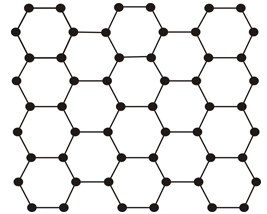
\includegraphics[scale=1]{Imagenes/Piezoelectricidad_01.png}
\end{figure}
\end{frame}
\begin{frame}
\begin{figure}
    \centering
    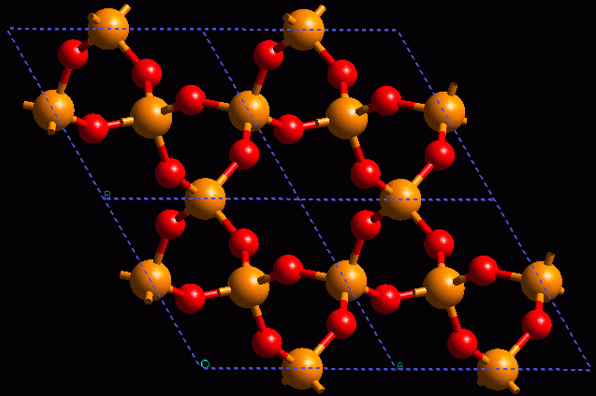
\includegraphics[scale=0.6]{Imagenes/Piezoelectricidad_02.png}
\end{figure}
\end{frame}

\subsection{Cerámicos}

\begin{frame}
\frametitle{¿Qué es un cerámico?}
Los materiales cerámicos son una clase de \textocolor{byzantium}{materiales inorgánicos sólidos} \pause que están formados principalmente por compuestos metálicos y no metálicos \pause unidos mediante enlaces iónicos o covalentes.
\end{frame}
\begin{frame}
\begin{figure}
    \centering
    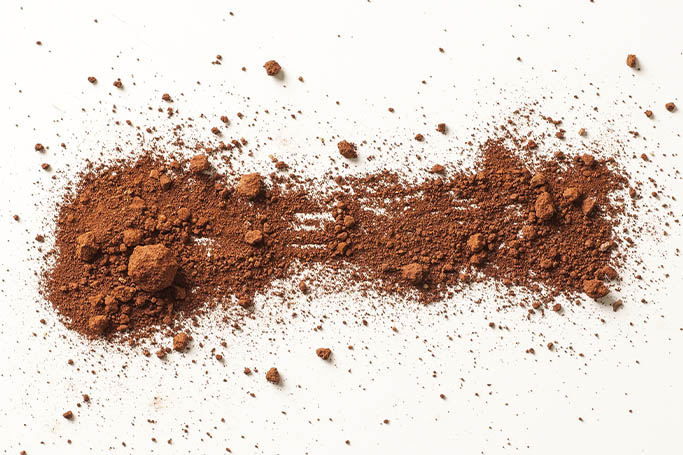
\includegraphics[scale=0.7]{Imagenes/Piezoelectricidad_03.jpg}
\end{figure}
\end{frame}
\begin{frame}
\frametitle{¿Qué es un cerámico?}
Estos materiales se caracterizan por su alta resistencia a la temperatura, \pause dureza, \pause resistencia a la corrosión, \pause y baja conductividad eléctrica y térmica.
\end{frame}

\subsection{Polímeros}

\begin{frame}
\frametitle{¿Qué es un polímero?}
Los polímeros son \textocolor{debianred}{macromoléculas} formadas por la repetición de unidades simples llamadas \textocolor{carmine}{monómeros}.
\end{frame}
\begin{frame}
\frametitle{¿Qué es un polímero?}
Estas unidades se unen mediante enlaces covalentes para formar largas cadenas o redes, lo que confiere a los polímeros propiedades únicas y diversas.
\end{frame}
% \begin{frame}
% \frametitle{Tipos de polímeros}
% \setbeamercolor{item projected}{bg=bananayellow,fg=black}
% \setbeamertemplate{enumerate items}{%
% \usebeamercolor[bg]{item projected}%
% \raisebox{1.5pt}{\colorbox{bg}{\color{fg}\footnotesize\insertenumlabel}}%
% }
% \begin{enumerate}[<+->]
% \item Polietileno (PE)
% % : El polietileno es uno de los plásticos más comunes y versátiles. Se utiliza en una amplia gama de aplicaciones, incluyendo envases de alimentos, bolsas de compras, botellas de plástico, aislantes eléctricos y tuberías.
% \item Poli(cloruro de vinilo) (PVC)
% % : El PVC es un plástico resistente y duradero que se utiliza en una variedad de aplicaciones, incluyendo tuberías, revestimientos para cables eléctricos, perfiles para ventanas y puertas, y productos de vinilo como suelos y revestimientos.
% \item Polipropileno (PP)
% % : El polipropileno es un plástico resistente al calor y a los productos químicos que se utiliza en una amplia variedad de aplicaciones, incluyendo envases de alimentos, componentes automotrices, textiles, y equipo médico.
% \seti
% \end{enumerate}
% \end{frame}
% \begin{frame}
% \frametitle{Tipos de polímeros}
% \setbeamercolor{item projected}{bg=bananayellow,fg=black}
% \setbeamertemplate{enumerate items}{%
% \usebeamercolor[bg]{item projected}%
% \raisebox{1.5pt}{\colorbox{bg}{\color{fg}\footnotesize\insertenumlabel}}%
% }
% \begin{enumerate}[<+->]    
% \conti
% \item Poliestireno (PS)
% % : El poliestireno es un plástico transparente y rígido que se utiliza en aplicaciones como envases de alimentos, utensilios desechables, bandejas de semillas, y material de embalaje.
% \item Poliéster (PET)
% % : El poliéster es un polímero resistente al calor y a los productos químicos que se utiliza en aplicaciones como fibras textiles (por ejemplo, para hacer ropa y alfombras), envases de alimentos, botellas de plástico y películas de embalaje.
% \item Poliuretano (PU)
% % : El poliuretano es un polímero flexible y resistente que se utiliza en una variedad de aplicaciones, incluyendo espumas para colchones y muebles, recubrimientos impermeables, adhesivos y sellos.
% \item Polimetilmetacrilato (PMMA)
% % : El PMMA es un polímero transparente y resistente a los impactos que se utiliza en aplicaciones como ventanas de acrílico, paneles de visualización, lentes ópticas y prótesis médicas.
% \end{enumerate}
% \end{frame}

\section{Piezoelectricidad}
\frame{\tableofcontents[currentsection, hideothersubsections]}
\subsection{Definición}

\begin{frame}
\frametitle{¿Qué es la piezoelectricidad?}
La \textocolor{red}{piezoelectricidad} es un fenómeno físico en el cual ciertos materiales tienen la capacidad de \textocolor{blue}{generar una carga eléctrica}.
\end{frame}
\begin{frame}
\frametitle{¿Qué es la piezoelectricidad?}
Cuando se someten a una \textocolor{coquelicot}{deformación mecánica} o una \textocolor{cadmiumgreen}{presión externa}, y viceversa.
\end{frame}
\begin{frame}
\frametitle{¿Qué es la piezoelectricidad?}
Este efecto se conoce como \textocolor{ao(english)}{efecto piezoeléctrico}.
\end{frame}    
\begin{frame}
\frametitle{El efecto piezoeléctrico}
\vspace*{-1cm}
\begin{figure}
    \centering
    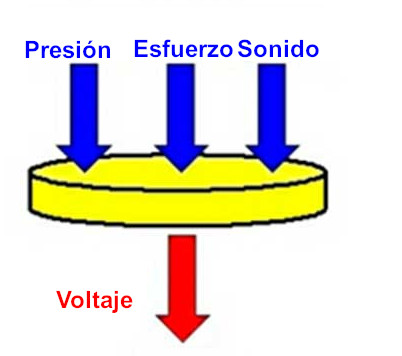
\includegraphics[scale=0.5]{Imagenes/Piezoelectricidad_04b.jpg}
\end{figure}
\end{frame}
\begin{frame}
\frametitle{El efecto piezoeléctrico}
\vspace*{-1cm}
\begin{figure}
    \centering
    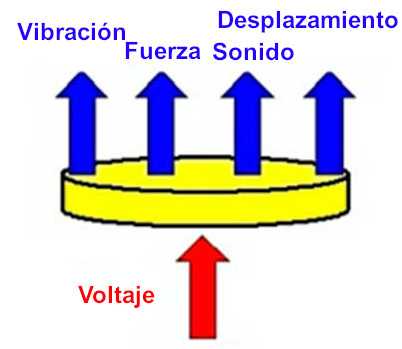
\includegraphics[scale=0.5]{Imagenes/Piezoelectricidad_04c.jpg}
\end{figure}
\end{frame}
\begin{frame}
\frametitle{¿Qué es la piezoelectricidad?}
Los materiales piezoeléctricos son aquellos que responden al efecto piezoeléctrico: \pause ciertos materiales cristalinos, cerámicos y poliméricos.
\end{frame}

\subsection{Materiales piezoeléctricos}

\begin{frame}
\frametitle{Cristales}
Un cristal piezoeléctrico es un tipo de material cristalino que exhibe el efecto piezoeléctrico.
\end{frame}
\begin{frame}
\frametitle{Cristales}
Este fenómeno se debe a la estructura asimétrica de los cristales piezoeléctricos, \pause que permite la separación y el movimiento de las cargas eléctricas dentro del material en respuesta a una tensión mecánica.
\end{frame}
\begin{frame}
\frametitle{Cristales}
Algunos de los cristales más comunes que exhiben propiedades piezoeléctricas son:
\setbeamercolor{item projected}{bg=buff,fg=black}
\setbeamertemplate{enumerate items}{%
\usebeamercolor[bg]{item projected}%
\raisebox{1.5pt}{\colorbox{bg}{\color{fg}\footnotesize\insertenumlabel}}%
}
\begin{enumerate}[<+->]
\item \textocolor{carminered}{Cuarzo}:

El cuarzo es uno de los cristales piezoeléctricos más utilizados.
\seti
\end{enumerate}
\end{frame}
\begin{frame}
\frametitle{Cristales}
Tiene una alta estabilidad dimensional y una respuesta rápida a los cambios en el campo eléctrico.
\end{frame}
\begin{frame}
\frametitle{Cristales}
Se utiliza en una amplia variedad de aplicaciones, incluyendo sensores, transductores ultrasónicos, relojes de cuarzo y dispositivos de filtrado.
\end{frame}
\begin{frame}
\frametitle{Cristales}
\setbeamercolor{item projected}{bg=buff,fg=black}
\setbeamertemplate{enumerate items}{%
\usebeamercolor[bg]{item projected}%
\raisebox{1.5pt}{\colorbox{bg}{\color{fg}\footnotesize\insertenumlabel}}%
}
\begin{enumerate}[<+->]
\item \textocolor{carminered}{Tourmalina}:

La tourmalina es otro cristal que exhibe propiedades piezoeléctricas.
\end{enumerate}
\end{frame}
\begin{frame}
\frametitle{Cristales}    
Se utiliza en aplicaciones como sensores de presión, dispositivos de generación de energía y dispositivos de control de vibración.
\end{frame}

\section{Transformación de energía}
\frame{\tableofcontents[currentsection, hideothersubsections]}
\subsection{Mecánica a eléctrica}

\begin{frame}
\frametitle{Mecánica a eléctrica}
Cuando se aplica una \textocolor{coolblack}{fuerza mecánica} o se produce \textocolor{darkmagenta}{una deformación} en un material piezoeléctrico, \pause los iones en la estructura cristalina del material se desplazan, \pause generando una diferencia de potencial eléctrico a través del material.
\end{frame}
\begin{frame}
\frametitle{Mecánica a eléctrica}    
Esa diferencia de potencial eléctrico se captura utilizando electrodos colocados en la superficie del material piezoeléctrico.
\end{frame}
\begin{frame}
\frametitle{Mecánica a eléctrica}
Creando así una corriente eléctrica que puede ser utilizada para alimentar dispositivos electrónicos,  almacenada en una batería u obtener una señal eléctrica de algún dispositivo.
\end{frame}
\begin{frame}
\frametitle{Mecánica a eléctrica}
\begin{figure}
    \centering
    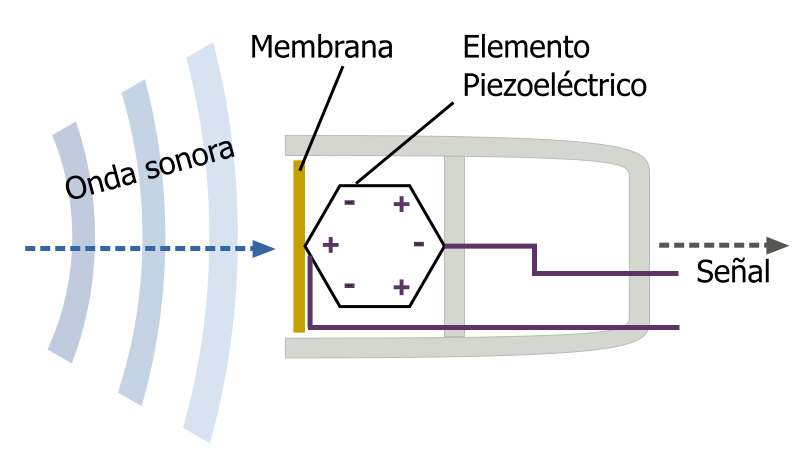
\includegraphics[scale=0.5]{Imagenes/Piezoelectricidad_05.png}
\end{figure}
\end{frame}

\subsection{Eléctrica a mecánica}

\begin{frame}
\frametitle{Eléctrica a mecánica}
Cuando se \textocolor{darkred}{aplica un campo eléctrico} externo a un material piezoeléctrico, \pause los \textocolor{deepcerise}{dipolos eléctricos} dentro del material se alinean, \pause causando una deformación o cambio en la forma del material.
\end{frame}
\begin{frame}
\frametitle{Eléctrica a mecánica}
Este proceso se utiliza en actuadores piezoeléctricos, \pause donde la aplicación de un voltaje eléctrico controlado permite ajustar o mover dispositivos mecánicos con gran precisión.
\end{frame}

\end{document}